\emph{Povodí} (\textit{drainage basin, watershed, catchment}) je území, ze kterého odtéká voda a sedimenty do jednoho vodního toku či jezera. Hranice povodí je nazývaná \emph{rozvodím}. K odtoku z povodí dochází v nejnižším bodě -- \emph{závěrovém profilu} (\textit{outlet}). 

Povodí jsou pro celou řadu studií (geomorfologických, hydrologických) základní jednotkou krajiny, na které se sleduje srážko-odtokový proces chod sedimentů ale také třeba jakým způsobem tyto procesy ovlivňují změny v hospodaření. 

Tvar povodí je ovlivněn celou řadou fyzickogeografických a geologických faktorů. Například ukloněním ker zemské kůry vznikají asymetrická povodí (jedna strana povodí je větší než druhá). 

% TODO: \usepackage{graphicx} required
\begin{figure}
	\centering
	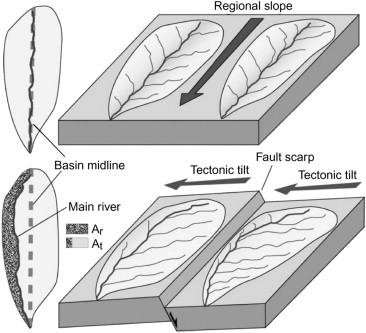
\includegraphics[width=1\linewidth]{obrazky/fluvial/watershed_tilt}
	\caption{Ukázka vzniku asymetrických údolí z důvodu tektonických pohybů. (zdroj \textcite{mahmoodAppraisalActiveTectonics2012})}
	\label{fig:watershedtilt}
\end{figure}

\section{Geometrie údolní sítě}
Uspořádání údolní sítě je výsledkem celé řady faktorů. Nejvýznamnější vliv má ale geologická struktura. \emph{Stromovitá údolní síť} má uspořádání toků podobné větvím stromu. Tento typ sítě se vyvíjí v oblastech tvořených z hornin podobné geomorfologické odolnosti. Vývoj sítě tak není ovlivněn litologií ale hlavně sklonem reliéfu. 
%
%\emph{Rovnoběžná údolní síť} má dlouhá údolí, která probíhají jedním směrem a jsou rovnoběžná. 
%
%\emph{Mřížkovitá údolní síť} se skládá z vodních toků dvou 

\begin{table*}[]
	\begin{tabularx}{\textwidth}{@{}llXX@{}}
		\toprule
		& Označení & Popis vzoru & Strukturní vliv \\ \midrule
		A & Stromovitá & Stromovitá struktura, hlavní tok vypadá kmen, přítoky větve. Bez zřejmého   usměrnění toků. & Horizontálně uložené sediment, homogení krystalické horniny, stejná   odolnost hornin. Bez vlivu geologických strukltur. \\
		B & Rovnoběžný & Hlavní toky jsou jednoho směru, rovnoběžné s pravidelnými rozestupy.   Přítoky se napojují pod ostrými úhly. & Zlomy v těsných rozestupech, monoklinální struktury nebo isoclinální   vrásy \\
		C & Mřížkovitý & Jeden hlavní směr toků. Sekundární směr je kolmý na hlavní. & Ukloněné nebo zvrásněné sedimentární horniny kde se střídají odolné a   neodolné jednotky. \\
		D & Pravoúhlý & Údolí tvoří pravoúhlou síť. Oba směry jsou rovnocenně zastoupeny. & Pukliny, zlomy \\
		E & Radiální & Vodní toky tečou od středu & Sopešné kužely, klenby \\
		F & Prstencovitý & Hlavní toky mají kruhový vzor, přítoky se napojují v pravých úhlech & Erodované klenby, kde se střídají odolné a neodolné jednotky \\
		G & Dostředný & Vodní toky tečou do středu & Kaldery, krátery, tektonické pánve \\
		H & Endoreický &  &  \\ \bottomrule
	\end{tabularx}
	\caption{Vzory říční sítě}
	\label{tab:ricni_sit}
\end{table*}


\section{Hiearchizace říční sítě}
Vodní toky v krajině rozdělujeme dle jejich řádu (Obr. \ref{fig:radtoku}). V hydrologii se běžně používá číslování \enquote{zespod nahoru}. Tedy postupuje se od toku, co ústí do moře. Tento tok je hlavní a označuje se jako tok I. řádu (např. Dunaj). Řeka Morava je pak II. řádu atd.

V geomorfologii se uplatňuje odlišné číslování \enquote{shora dolů}. Postupuje se od nejmenších toků v pramenných oblastech do nižších poloh ke stále větším tokům. Na tomto principu je založená Strahlerova nebo Shrevova klasifikace. \emph{Strahlerova klasifikace} říká, že spojením toků stejného řádu vzniká tok o jeden řád vyšší (např. spojením toků prvního řádu vzniká tok druhého řádu). Při soutoku řek odlišných řádů (např. 1. a 2.) zůstává zachován nejvyšší řád. \emph{Shrevova klasifikace} na soutocích řády sčítá. Tedy soutok dvou řek 1. řádu dá tok 2. řádu, soutok 3. a 1. řádu dá tok 4. řádu. 

% TODO: \usepackage{graphicx} required
\begin{figure}
	\centering
	\includegraphics[width=1\linewidth]{obrazky/fluvial/rad_toku}
	\caption{Klasická, Strahlerova a Shrevova hierarchizace říční sítě.}
	\label{fig:radtoku}
\end{figure}


\section{Jezera}
\emph{Jezera} jsou přirozené akumulace vody ve sníženinách na pevnině, které nejsou přímo spojené se světovým oceánem. Zaujímají přibližně $1,8 \%$ souše. Jezera jsou místní erozní bází, tudíž se toky nad jezerem nemohou zahlubovat pod úroveň jezera. Z dlouhodobého hlediska jsou jezera jen přechodným prvkem v krajině, neboť postupem času dochází k jejich zanesení sedimenty. 

Jedna z klasifikací jezer je podle jejich vzniku. Rozlišujeme tak:
\begin{itemize}
	\item Tektonická jezera	
	\item Vulkanická jezera
	\item Ledovcová jezera
	\item Sesuvová jezera
	\item Jezera vzniklá rozpouštěním
	\item Fluviální jezera
	\item Limanová jezera
	\item Jezera vzniklá rozpouštěním
	\item Jezera činností organismů
	\item Meteoritická jezera
\end{itemize}

Tvar jezerních pánví často odpovídá jejich genezi. Kruhový či oválný tvar mají jezeera vulkanická, závrtová nebo alasová. Jezera vzniklá v důsledku tektonických pohybů mají pravoúhlý tvar. Mrtvá ramena mají srpovitý tvar.


U velkých jezer vznikají jezerní terasy,





\newpage
\onecolumn
\begin{boxotazky}{Kontrolní a klíčové otázky, na které bychom měli znát odpověď}
	\begin{itemize}
		\item 
		\item 
		
	\end{itemize}
\end{boxotazky}

\begin{boxslovnik}{Další klíčové pojmy k zapamatování}
	aaa & adfasd \\
	
\end{boxslovnik}
\twocolumn

